\chapter{Разработка адаптивного к скорости метода управления ДРК ПА}\label{ch:Allocation}

\section{Формальное описание структуры ДРК}\label{sec:Allocation/System}
\begin{noteplan}
	Думаю эту секцию перенесу во вторую главу. А здесь оставлю только анализ матрицы геометрии ДРК.
\end{noteplan}

Движители в системе можно разделить на три больших класса \cite{армишев86}:
\begin{itemize}
    \item \textbf{фиксированные}, когда вектор упора может изменяться только вдоль фиксированной относительно ПА прямой.
    \item \textbf{поворотные} (азимутальные, azimuth), когда вектор упора может изменяться в фиксированной относительно ПА плоскости.
    Сюда относятся гребные винты на поворотных колонках, гребные винты с поворотными насадками, крыльчатые движители и т.д.
    \item \textbf{пространственные}, когда вектор упора может изменяться в пространстве.
\end{itemize}
Следует отметить, что если первые два класса движителей были заимствованы для ПА с надводных судов, то пространственные движители были разрабтаны для решения специфических задач подводных аппаратов.

Определим формально, как по структуре ДРК находится число степеней свободы $m$, которые можно контролировать движение данного ПА, и наоборот, какова должна быть структура ДРК, что бы можно было управлять по заданным степеням свободы.

Пусть $Oxyz$ -- правая ортогональная система координат жестко связанная с ПА. Ось $Ox$ направлена из кормы в нос, ось $Oy$ с левого борта на правый, а ось $Oz$ дополняет систему до правой ортогональной (SNAME нотация системы координат).

Введём следующие обозначения:
\begin{itemize}
    \item $n_f \geq 0, n_a \geq 0, n_r \geq 0$ -- число, соответственно, фиксированных, поворотных и пространственных движителей входящих в состав ДРК;
    % \item $i$ -- номер по порядку каждого движителя, где $i$ меняется в диапазоне $1,2, \ldots, n_f+n_a+n_r$;
    \item $u^{i}, i < n_f$ - величина упора фиксированного движителя;
    \item $(u^{i}_x, u^{i}_y, u^{i}_z)$, где $i$ меняется в диапазоне $n_f+1, n_f+2, \ldots, n_f+n_a+n_r$ -- проекции векторов упоров поворотных и пространственных движителей, соответственно на оси $Ox, Oy, Oz$;
    \item $(P^i_x, P^i_y,P^i_z)$ -- координаты точки крепления движителя с номером $i$ относительно $Oxyz$;
    \item $(C^i_x, C^i_y, C^i_z)$ -- направляющие косинусы единичного вектора, направленного вдоль линии действия фиксированного движителя с номером $i$;
    \item $(R^i_x, R^i_y, R^i_z)$, где $i$ меняется в диапазоне $n_f+1, n_f+2, \ldots, n_f+n_a$ -- направляющие косинусы вектора единичной нормали к плоскости вращения поворотного движителя с номером $i$;
    \item $(\nu_x, \nu_y, \nu_z)$ -- проекции главного вектора управляющих сил на оси $Ox, Oy, Oz$;
    \item $(\nu_{mx},\nu_{my},\nu_{mz})$ -- проекции главного вектора момента управляющих сил на оси $Ox, Oy, Oz$.
    \item $\vect{u}=[u^{1}, u^{2}, \ldots, u^{n_f+n_a+n_r}_x, u^{n_f+n_a+n_r}_y, u^{n_f+n_a+n_r}_z]^T$ -- обобщенный вектор упоров создаваемый ДРК;
    \item $\vect{\nu} = [\nu_x, \nu_y, \nu_z, \nu_{mx},\nu_{my},\nu_{mz}]^T$ -- обобщенный вектор сил и моментов действующий на аппарат в системе координат $Oxyz$.
\end{itemize}

Можно показать что между векторами $\vect{u}$  и $\vect{\nu}$ есть линейная зависимость, которая выражается через матрицу $B$:
\begin{equation}
    \label{eq:propulsion_connection}
    B\vect{u} = \vect{\nu}
\end{equation}

В \ref{eq:propulsion_connection} шесть уравнений определяют связь между проекциями сил и моментов в связанной с аппаратом системе координат $Oxyz$ с одной стороны и $n_f$ упоров фиксированных и $3(n_r+n_r)$ проекций упоров поворотных и пространственных движителей с другой стороны.

Однако не все создаваемые движителями упоры являются независимыми.
Вектор тяги поворотного движителя должен всегда лежать в плоскости вращения. 
Для этого вводят расширенный вектор сил и моментов $\vect{\nu^e} = [\vect{\nu}, 0, \ldots, 0]$, где $\vect{\nu^e} \in \mathspace{R}^{6+n_a}$ и соответствующую матрицу $B^e$:
\begin{equation}
    \label{eq:propulsion_connection_enchanced}
    B^e\vect{u} = \vect{\nu^e}
\end{equation}
где последние $n_a$ уравнений отражают это ограничение накладываемое на вращательные движители.

Общие вид матрицы $B^e=(B^e_f, B^e_a, B^e_r)$, где $B^e_f \in \mathspace{R}^{(6 + n_f) \times n_f}$ (\ref{eq:propulsion_matrix_fix}), $B^e_a \in \mathspace{R}^{(6 + n_f) \times 3n_a}$ (\ref{eq:propulsion_matrix_azimuth}), $B^e_r \in \mathspace{R}^{(6 + n_f) \times 3n_r}$ (\ref{eq:propulsion_matrix_rotation}) -- матрицы отражающая влияние фиксированных движителей, поворотных и пространственных движителей соответственно.

\begin{equation}
    \label{eq:propulsion_matrix_fix}
    B^e_f = 
    \begin{pmatrix}
        C^1_x & \ldots & C^{n_f}_x \\
        C^1_y & \ldots & C^{n_f}_y \\
        C^1_z & \ldots & C^{n_f}_z \\
        [C^1 \times P^1]_x & \ldots & [C^{n_f} \times P^{n_f}]_x \\
        [C^1 \times P^1]_y & \ldots & [C^{n_f} \times P^{n_f}]_y \\
        [C^1 \times P^1]_z & \ldots & [C^{n_f} \times P^{n_f}]_z \\
        \ldots & \ldots & \ldots \\
        0 & \ldots & 0 \\
    \end{pmatrix}
\end{equation}

\begin{equation}
    \label{eq:propulsion_matrix_azimuth}
    B^e_a = 
    \begin{pmatrix}
        1 & 0 & 0 & \ldots & 1 & 0 & 0 \\
        0 & 1 & 0 & \ldots & 0 & 1 & 0 \\
        0 & 0 & 1 & \ldots & 0 & 0 & 1 \\
        0 & -P_z^1 & P_y^1 & \ldots & 0 & -P_z^{n_a} & P_y^{n_a} \\
        P_z^1 & 0 & -P_x^1 & \ldots & P_z^{n_a} & 0 & -P_x^{n_a} \\
        -P_y^1 & P_x^1 & 0 & \ldots & -P_y^{n_a} & P_x^{n_a} & 0 \\
        R_x^1 & R_y^1 & R_z^1 & \ldots & 0 & 0 & 0 \\
        \ldots & \ldots & \ldots & \ldots & \ldots & \ldots & \ldots \\
        0 & 0 & 0 & \ldots & R_x^{n_a} & R_y^{n_a} & R_z^{n_a} \\
    \end{pmatrix}
\end{equation}

\begin{equation}
    \label{eq:propulsion_matrix_rotation}
    B^e_r = 
    \begin{pmatrix}
        1 & 0 & 0 & \ldots & 1 & 0 & 0 \\
        0 & 1 & 0 & \ldots & 0 & 1 & 0 \\
        0 & 0 & 1 & \ldots & 0 & 0 & 1 \\
        0 & -P_z^1 & P_y^1 & \ldots & 0 & -P_z^{n_a} & P_y^{n_a} \\
        P_z^1 & 0 & -P_x^1 & \ldots & P_z^{n_a} & 0 & -P_x^{n_a} \\
        -P_y^1 & P_x^1 & 0 & \ldots & -P_y^{n_a} & P_x^{n_a} & 0 \\
        R_x^1 & R_y^1 & R_z^1 & \ldots & 0 & 0 & 0 \\
        \ldots & \ldots & \ldots & \ldots & \ldots & \ldots & \ldots \\
        0 & 0 & 0 & \ldots & 0 & 0 & 0 \\
    \end{pmatrix}
\end{equation}

Матрица $B^e$ зависит от расположения и ориентации движителей, а её размеры от числа различных типов движителей.
Следовательно она зависит только от структуры ДРК, в связи с чем будем её называть -- \textbf{матрицей структуры движительно-рулевого комплекса подводного аппарата}.
Формально многие вопросы, связанные с выбором структуры ДРК, могут быть решены с помощью матрицы структуры ДРК.

Элементы матрицы зависят от выбора системы координат.
Легко проверить, что в общем случае ортогонального преобразования (поворот и параллельный перенос) перевода в новую систему координат, когда произвольный вектор $\vect{v}=[v_x,v_y,v_z]^T$ переходит в $\vect{q}=[q_x,q_y,q_z]^T$:
\begin{equation*}
    \left\{
    \begin{array}{ll}
         &\vect{q} = R\vect{v} + \vect{d}\\
         &\det[R] = 1
    \end{array}
    \right.
\end{equation*}
\noindent где $R$ -- матрица поворота, $\vect{d}$ -- вектор линейного переноса в систему координат $(Oxyz)')$.

Матрица $B^e$ в новой системе координат будет задана следующим образом:
\begin{equation}
    B^e_{(Oxyz)'} = Q_2Q_3B^eQ_1
\end{equation}
\noindent где $B^e_{(Oxyz)'}$ -- матрица конфигурации ДРК в новой системе координат, $Q_1 \in \mathspace{R}^{(n_f+3n_a+3n_r)\times(n_f+3n_a+3n_r)}$ (\ref{eq:matrix_rotation_q1}), $Q_2 \in \mathspace{R}^{(6+n_a)\times(6+n_a)}$ (\ref{eq:matrix_rotation_q2}), $Q_3 \in \mathspace{R}^{(6+n_a)\times(6+n_a)}$ (\ref{eq:matrix_rotation_q3}) -- диагональные матрицы перехода в $(Oxyz)'$.

\begin{equation}
    \label{eq:matrix_rotation_q1}
    Q_1 = 
    \setlength{\arraycolsep}{0pt}
    \begin{pNiceMatrix}[columns-width=auto]
        I^{n_f\times n_f} &     &         & \text{\Large0} \\
                          & R^T &         &                \\
                          &     & \ddots  &                \\
        \text{\Large0}    &     &         & R^T
    \end{pNiceMatrix}
\end{equation}
\noindent где:
\begin{itemize}
    \item $I^{n_f\times n_f} \in \mathspace{R}^{n_f \times n_f}$ -- единичная диагональная матрица;
\end{itemize}

\begin{equation}
    \label{eq:matrix_rotation_q2}
    Q_2 = 
    \setlength{\arraycolsep}{0pt}
    \begin{pNiceMatrix}[columns-width=auto]
        R               &     &         & \text{\Large0} \\
                        & R   &         &                \\
                        &     & \ddots  &                \\
        \text{\Large0}  &     &         & I^{n_a\times n_a}
    \end{pNiceMatrix}
\end{equation}

\begin{equation}
    \label{eq:matrix_rotation_q3}
    Q_3 = 
    \setlength{\arraycolsep}{0pt}
    \begin{pNiceMatrix}[columns-width=auto]
        W & 0 \\
        0 & I^{n_a \times n_a}
    \end{pNiceMatrix}
\end{equation}

\noindent где матрица $W$ определяется следующим выражением:
\begin{equation*}
    \setlength{\arraycolsep}{0pt}
    \begin{pNiceMatrix}[columns-width=auto]
        1    & 0    & 0    & 0 & 0 & 0 \\
        0    & 1    & 0    & 0 & 0 & 0 \\
        0    & 0    & 1    & 0 & 0 & 0 \\
        0    & -d_z & d_y  & 1 & 0 & 0 \\
        d_z  & 0    & -d_x & 0 & 1 & 0 \\
        -d_y & d_x  & 0    & 0 & 0 & 1
    \end{pNiceMatrix}
\end{equation*}

По виду матриц $Q_1, Q_2, Q_3$ следует что их определители совпадают и равны единице:
\begin{equation*}
    \det Q_1 = \det Q_2 = \det Q_3 = 1
\end{equation*}

Отсюда следует что при ортогональном преобразовании ранг матрицы ДРК $B^e$ не изменяется:
\begin{equation*}
    \text{rg}B^e = \text{rg}B^e_{(Oxyz)'} = \text{const}
\end{equation*}

Рассмотрим как связаны свойства матрицы структуры движительно-рулевого комплекса ПА с возможностью управления по заданным степеням свободы.
Это означает, что данный ДРК может одновременно создавать заданные вектора управляющей силы и момента или только некоторых из их проекций.
Так, например, для управления по четырем степеням свободы (продольное и вертикальное перемещение, курс, дифферент), необходимо что бы ДРК создавал две заданные проекции управляющей силы и две проекции момента.
Необходимое число контролируемых степеней свободы существенно зависит от целевых задач ПА. 

Для необитаемых ПА необходимо создавать достаточно сложные ДРК, способные управлять по 5-6 степеням свободы.
На обитаемых ПА, как правило, управляют по четырем степеням свободы (вперед, вверх, лаг, курс).
Для управления же по крену и дифференту на обитаемых ПА чаще используются перемещаемые грузы или жидкости -- крен-дифферентные системы.
Однако, и на обитаемых ПА в ряде случаев требуются высокоточное управление по всем шести степеням свободы.

Рассмотрим наиболее сложные структуры ДРК, предназначенные для управления по шести степеням свободы ($m=6$).
Ранг матрицы структуры ДРК должен удовлетворять условию:
\begin{equation}
    \label{eq:propulsion_matrix_rank}
    \text{rg}B^e=6+n_a
\end{equation}
Причём данное условие является необходимым и достаточным.
То есть, если данный ДРК способен управлять одновременно по $m=6$ степеням свободы, то его матрица структуры удовлетворяет данному условию и наоборот.

В общем случае для $m\leq 6$ аналогичное условие будет записано следующим образом:
\begin{equation}
    \label{eq:propulsion_matrix_rank_com}
    \text{rg}B^e \geq m + n_a
\end{equation}

Пусть $m=6$ и требуется создать вектор сил и моментов $\vect{\nu}$.
Для решения задачи распределения вектора упоров между движителями необходимо решить систему линейных уравнений \ref{eq:propulsion_connection}.
При этом можно показать что при выполнении условия \ref{eq:propulsion_matrix_rank_com} решение системы \ref{eq:propulsion_connection} всегда существует, однако может быть не единственным.
Это означает что заданную управляющую силу можно создать при различных сочетаниях векторов упоров на движителях.
Такие ДРК называются \textbf{избыточными}, в отличие от неизбыточных, когда распределение упоров можду движителями может быть единственным.
избыточные ДРК могут применяться и для управляения по меньшему числу степеней свободы $m \leq 6$.

Формально вопрос избыточности ДРК решаетя по виду матрицы $B^e$.
Как нетрудно установить, ДРК будет неизбыточным для управления по $m=6$ степеням свободы, когда матрица $B^e$ квадратная и выполняется условие \ref{eq:propulsion_matrix_rank}, то есть:
\begin{equation}
    \left\{
    \begin{array}{ll}
    n_f + 2n_a + 3n_r = 6  \\
    \det B^e \neq 0 
    \end{array}
    \right.
\end{equation}
\noindent и избыточным в случае:
\begin{equation}
    \left\{
    \begin{array}{ll}
    n_f + 2n_a + 3n_r > 6  \\
    \text{rg}B^e = 6 + n_a
    \end{array}
    \right.
\end{equation}

В общем случае для $m \leq 6$ неизбыточные ДРК определяются следующим образом:
\begin{equation}
    \left\{
    \begin{array}{ll}
    n_f + 2n_a + 3n_r = N  \\
    \text{rg}B^e = N + n_a
    \end{array}
    \right.
\end{equation}
\noindent а избыточные:
\begin{equation}
    \left\{
    \begin{array}{ll}
    n_f + 2n_a + 3n_r > \text{rg}B^e  \\
    \text{rg}B^e \geq N + n_a
    \end{array}
    \right.
\end{equation}

\section{Учет рулей управления в матрице структуры ДРК ПА}
\begin{noteplan}
	Эта часть еще сырая, буду её серьезно перерабатывать.
\end{noteplan}
Уравнение \ref{eq:propulsion_connection} не поддерживает рули управления как один из способов контроля движения ПА.
Это исторически отдельная задача и ей посвящено достаточно много литературы в области управления летательными аппаратами, но рули управления также широко распространены и в подводных аппаратах, и задача распределения управляющих воздействий между этими исполнительными механизмами остаётся актуальной.

Так например в работе \cite{10.1177/1729881417741738} закон линейной взаимосвязи между обобщенным вектором силы и момента в связанной системе координат BODY $\vect{\nu}$ и вектором углов поворота движителей $\vect{\delta}$, определяется следующим образом:
\begin{equation}
    \begin{pmatrix}
        X \\
        Y \\
        Z \\
        K \\
        M \\
        N
    \end{pmatrix}
    = u^2
    \begin{pmatrix}
        X_{\delta_1\delta_1} & X_{\delta_2\delta_2} & X_{\delta_3\delta_3} & X_{\delta_4\delta_4} \\
        Y_{\delta_1} & Y_{\delta_2} & Y_{\delta_3} & Y_{\delta_4} \\
        Z_{\delta_1} & Z_{\delta_2} & Z_{\delta_3} & Z_{\delta_4} \\
        K_{\delta_1} & K_{\delta_2} & K_{\delta_3} & K_{\delta_4} \\
        M_{\delta_1} & M_{\delta_2} & M_{\delta_3} & M_{\delta_4} \\
        N_{\delta_1} & N_{\delta_2} & N_{\delta_3} & N_{\delta_4}
    \end{pmatrix}
    \begin{pmatrix}
        \delta_1 \\
        \delta_2 \\
        \delta_3 \\
        \delta_4
    \end{pmatrix}
\end{equation}
\noindent
\begin{itemize}
    \item $\nu = [X, Y, Z, K, M, N]^T$ -- обобщенный вектор сил вдоль продольной, поперечно и нормальной осью ССК, и моментов вокруг них;
    \item $\vect{\delta} = [\delta^1, \delta^2, \delta^3, \delta^4]^T$ -- вектор углов поворота рулей, где $\delta^1, \delta^2, \delta^3, \delta^4$ -- углы поворота соответственно верхнего левого, верхнего правого, нижнего левого и нижнего правого кормового руля управления;
    \item $u$ -- скорость потока воды набегаемой на аппарат при его движении;
    \item $X_{\delta_i, \delta_i}, \ldots, N_{\delta_i}$ -- коэффициент сил и моментов создаваемых РУ при скорости набегаемого потока $u$.
\end{itemize}

\section{Формирование фиксированных пропорций значений целевого управления}\label{sec:Allocation/System}

\section{Метод адаптивного управления ДРК ПА} \label{sec:Allocation/Method}

\subsection{Задача оптимального управления ДРК ПА}
\begin{notequestion}
	Заново постановка задачи оптимального управления ДРК. Для тех кто забыл всё из первой главы пока до сюда добрался.
	Может и не писать?
\end{notequestion}
Согласно выражению \ref{eq:Statement/AllocationProblem} задача оптимального управления ДРК ПА ставится следующим образом:

\begin{equation}
	\label{eq:Allocation/Problem}
	\begin{matrix}
		\min \left( ||Q_s|| + J(\vect{x}, \vect{u}, t) \right) \\
		\text{при условии } \\
    	\vect{\nu}-B(\vect{x})\vect{u} = \vect{s}, u \in \mathspace{U}
	\end{matrix}
\end{equation}
\noindent где:
\begin{itemize}
	\item $\vect{\nu}$ -- целевой вектор виртуального управления;
	\item $\vect{u}$ -- вектор управления исполнительными механизмами;
	\item $B$ -- матрица геометрии движительно-рулевого комплекса;
    \item $s$ -- невязку вектора виртуального управления, которая определяет меру различия между заданным и сформированным вектором управления;
    \item $Q_{\nu}$ -- матрица, формализующая приоритеты работы тех или иных осей управления при выходе вектора $\nu$ за пределы допустимого множества $\mathspace{A}$.
    \item $J(\vect{x}, \vect{u}, t)$ -- некоторый функционал качества.
\end{itemize}

В разделе \ref{sec:Statement/Methods} перечислены различные методы используемые для решения задачи управления избыточного ДРК ПА, как оптимальные так и нет.
Все методы имеют свои преимущества и недостатки.

\subsection{Решение задачи оптимизации через теорему о сжимающем прострастве}

\begin{noteplan}
	Это пока ядро метода. Ещё будет добавлена модификация матрицы в случае подруливающих движителей, рулей и добавлена матрица отказоустойчивости.
\end{noteplan}

В рамках исследования было предложено использовать новый математический метод решения задачи управления ДРК в рамках которого поиск минимума  $J(\vect{x}, \vect{u}, t)$ может быть сформулирован через теорему о неподвижной точке в сжимающем пространстве \cite{rhoades2004quadratic}, который было предложено применять для рулей управления АНПА в работе \cite{zhang2017design}.

Пусть функционал $J(\vect{x}, \vect{u}, t)$ задан в рамках минимазации потребления энергии исполнительными механизмами ДРК следующим образом \cite{burken2001two}:
\begin{equation}
    J = (1-\varepsilon)(B\vect{u} - \vect{\nu})^TQ_1(B\vect{u} - \vect{\nu}) + \varepsilon 
    \vect{u}^TQ_2\vect{u}
\end{equation}
\noindent где:
\begin{itemize}
    \item $\varepsilon$ -- некоторый множитель меньше 1;
    \item $Q_{\nu}=W^T_{\nu}W_{\nu}$, где $W_{\nu}$ -- диагональная матрица положительно определенных весовых коэффициентов осей управления;
    \item $Q_{u}=W^T_{u}W_{u}$, где $W_u$ -- диагональная матрица положительно определенных весовых коэффициентов ИМ;
\end{itemize}

Тогда инеративное решение оптимизационной задачи \ref{eq:Allocation/Problem} может быть найдено следующим образом:
\begin{equation}
	\label{eq:Allocation/FixedMethod}
    \vect{u}_{n+1} = \text{sat}
    \left[
    (1-\varepsilon)\omega B^TQ_{\nu}\nu - (\omega H - I) \vect{u}_{n}
    \right]
\end{equation}
\noindent где:
\begin{itemize}
	\item $H=(1 - \varepsilon)B^TQ_1B + \varepsilon Q_2$;
	\item $\omega = 1 / ||H||_2$;
	\item $I$ -- диагональная единичная матрица;
	\item $\vect{u}_{n+1}$ -- вектор управления исполнительными механизмами на $\vect{u}$ шаге итерационного расчёта.
\end{itemize}

Функция $\text{sat}(x)$ определяет поведение выражения \ref{eq:Allocation/FixedMethod} при $\vect{u} \notin \mathspace{U}$ следующим образом:
\begin{equation*}
	\text{sat}(x) = 
	\left\{
	\begin{array}{lll}
		u^{min}, &&x < u^{min} \\
		x,         &u^{min} < &x < u^{max} \\
		u^{max}, &u^{max} < &x 
	\end{array}
	\right.
\end{equation*}

Итеративный расчёт вектора $\vect{u}_{n}$ заканчивается при выполнении следующего неравенства:
\begin{equation*}
	\left| J(\vect{u}_{k+1}) - J(\vect{u}_{k}) \right| < J_{end}
\end{equation*}
\noindent где $J_{end}$ -- настраиваемый параметр, который зависит от дискретности управления исполнительными механизмами ДРК.

\begin{notequestion}
	По-хорошему, надо задать конкретные правила формирования $J_{end}$.
\end{notequestion}
\section{Сравнительный анализ основных параметров работы метода адапативного управдения ДРК ПА} \label{sec:Allocation/Compare}
\begin{noteplan}
	Тут будет сравнительная характеристика различных подходов. Как в статье на УМС.
\end{noteplan}

\section{Моделирование работы предлагаемого метода управления ДРК при различных скоростях набегающего потока} \label{sec:Allocation/Test}

\begin{noteplan}
	Тут я по сути пока вставил просто картинки. Потом подробнее опишу методологию модельного эксперимента.
\end{noteplan}

Численное моделирование разработанного алгоритма проводилось на модели АНПА ``ММТ-300'' спроектированного и разработанного в ИПМТ ДВО РАН.
Он оснащен четырьмя маршевыми движителями, расположенными в корме аппарата и двумя подруливающими движителями - в горизонтальной и вертикальной плоскостях.
Положение и ориентация каждого движителя представлена в таблице \ref{tab:mmt300_propulsion}.
В таблице \ref{tab:mmt300_propulsion} уголы $\psi$ и $\theta$ определяют отклонение вектора формирования упора движителя от продольной оси аппарата в горизонтальной и вертикальной плоскости соответственно.
Координата в ССК определяет положение движителя в системе координат связанной с ЦМ ПА, где ось $x$ направлена вдоль продольной оси аппарата с кормы в нос, ось $y$ направлена вдоль поперечной оси аппарата от левого бока на правый и ось $z$ достраивает СК до правосторонней.

\begin{figure}[ht]
    \centering
    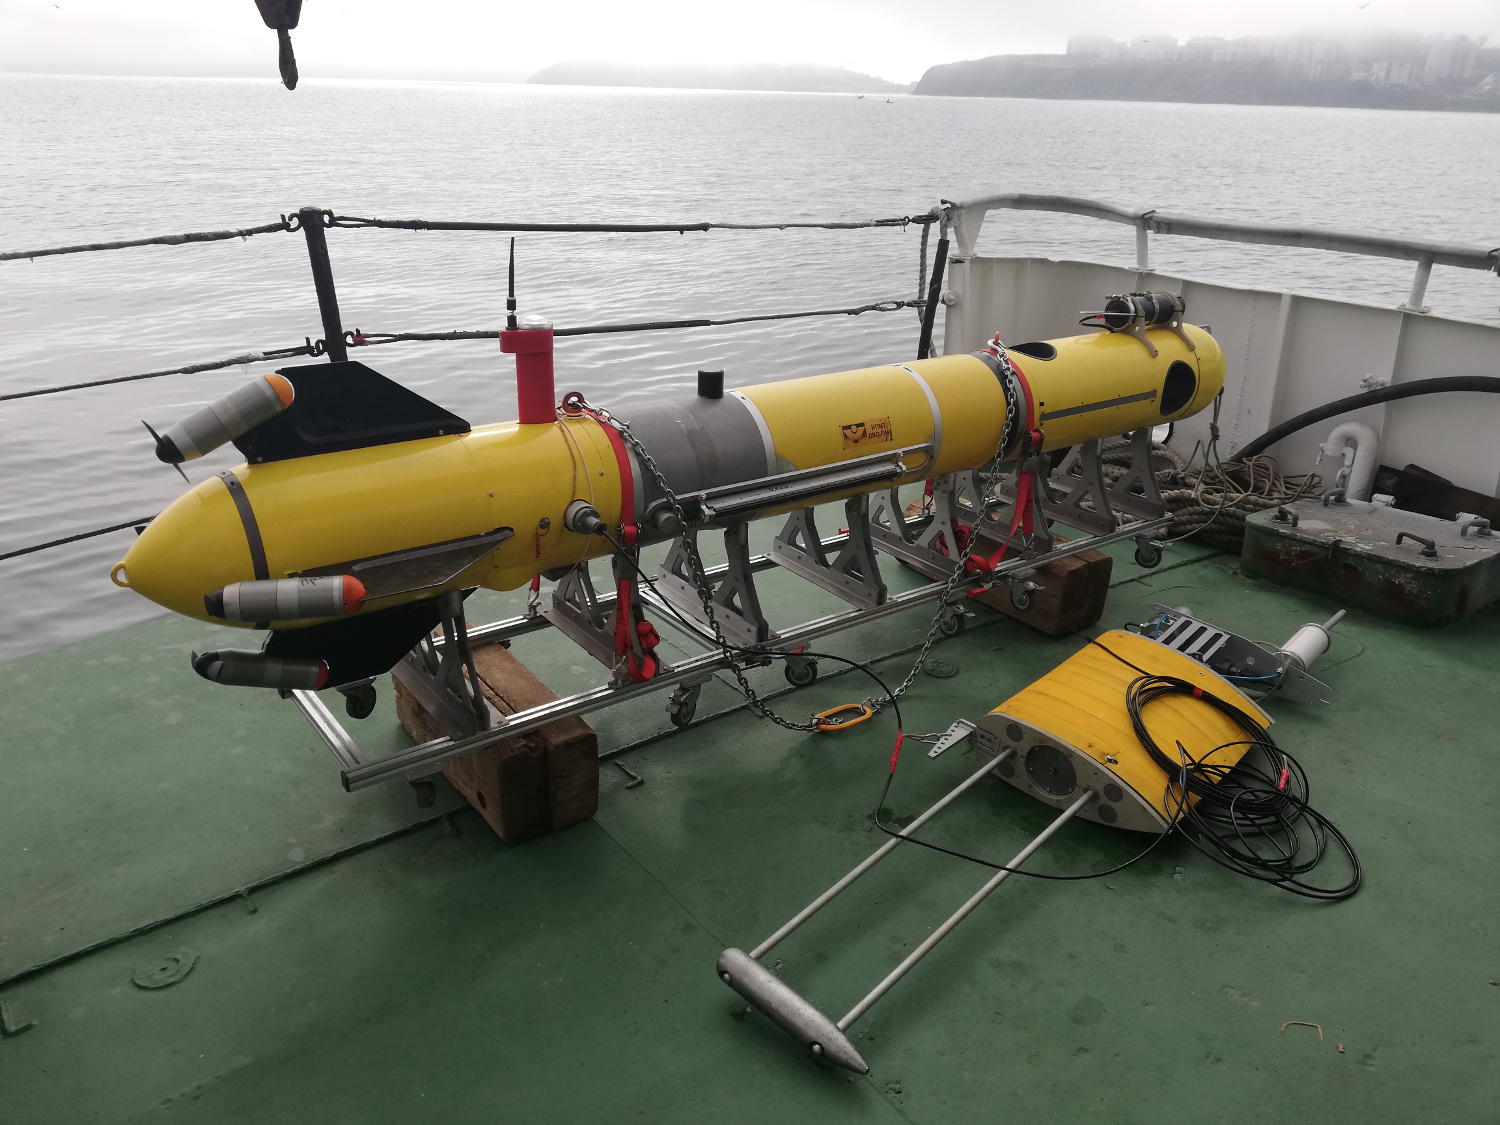
\includegraphics[width=0.8\linewidth]{allocation/Распределение - вид ММТ300.jpg}
    \caption{Общий вид аппарата АНПА ``ММТ-300''.}
    \label{fig:mmt-300}
\end{figure}

\begin{table}
    \caption{Параметры ДРК АНПА ``ММТ-300''.}
    \label{tab:mmt300_propulsion}
    \centering
    \begin{tabular}{lll}
        \toprule
        Тип движителя & \makecell[l]{Пространственная ориентация \\ $(\psi, \theta)$, $^{\circ}$} & \makecell[l]{Координата в ССК \\ 
        $(x,y,z)$, м} \\
        \midrule
        Левый   кормовой & (-22.5, 0) & (-1.60,-0.14,0) \\
        Правый  кормовой & (22.5, 0)  & (-1.60,0.14,0) \\
        Нижний  кормовой & (0, -22.5) & (-1.60,0,0.14) \\
        Верхний кормовой & (0, 22.5)  & (-1.60,0,-0.14) \\
        \makecell[l]{Подруливающий \\ вертикальный}   & (0, 90) & (0.3,0.0,0,0) \\
        \makecell[l]{Подруливающий \\ горизонтальный} & (90, 0) & (1.0,0.0,0,0) \\
        \bottomrule
    \end{tabular}
\end{table}

В рамках исследования было произведено сравнение работы предлагаемого метода с методом распределения управляющего воздействия, который реализован на АНПА ``ММТ-300'' и описан в разделе \ref{sssec:AllocationFix}.

\begin{figure}[ht]
    \centering
    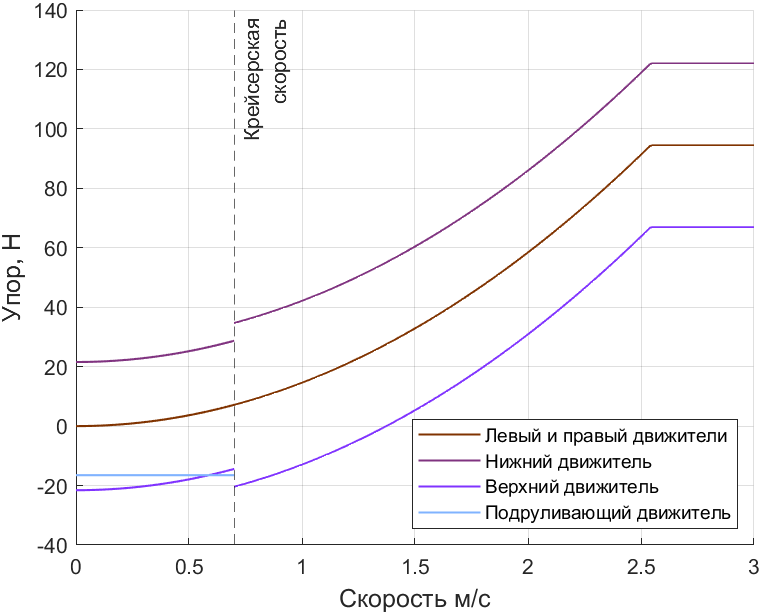
\includegraphics[width=0.8\linewidth]{allocation/Результат - Стандартный упоры.png}
    \caption{Распределение управления методом прямого распределения с масштабированием.}
    \label{fig:mmt-300-allocation-fix-thrust}
\end{figure}

\begin{figure}[ht]
    \centering
    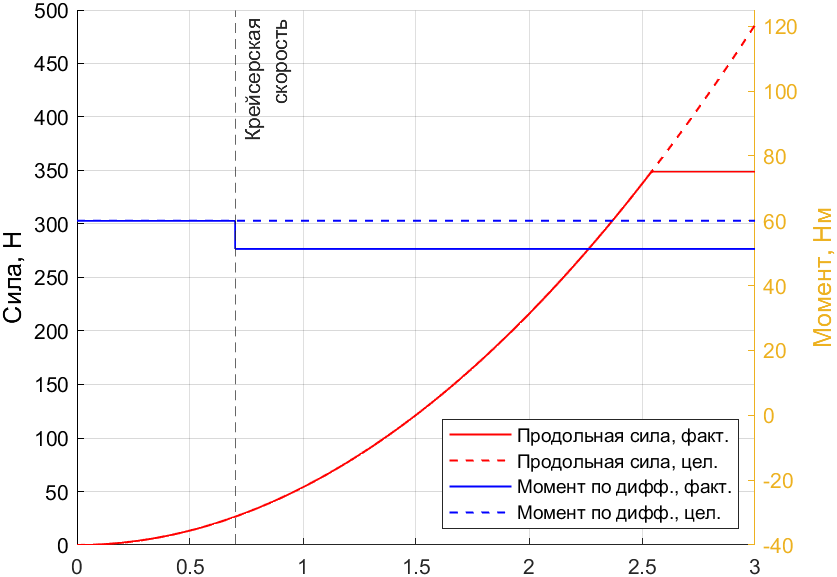
\includegraphics[width=0.8\linewidth]{allocation/Результат - Стандартный силы.png}
    \caption{Силы и моменты при прямом распределении с масштабированием.}
    \label{fig:mmt-300-allocation-fix-force}
\end{figure}

\begin{figure}[ht]
    \centering
    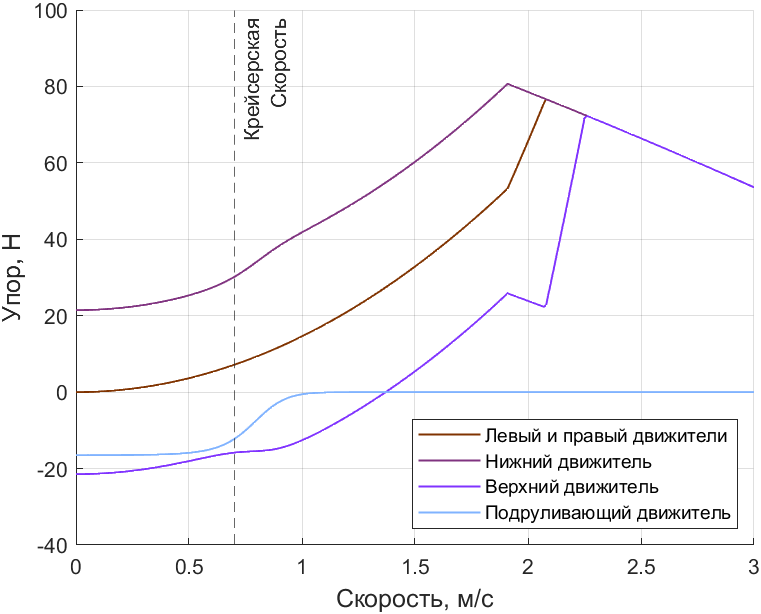
\includegraphics[width=0.8\linewidth]{allocation/Результат - Адаптивный Упоры.png}
    \caption{Распределение управления предлагаемым методом.}
    \label{fig:mmt-300-allocation-optimal-thrust}
\end{figure}

\begin{figure}[ht]
    \centering
    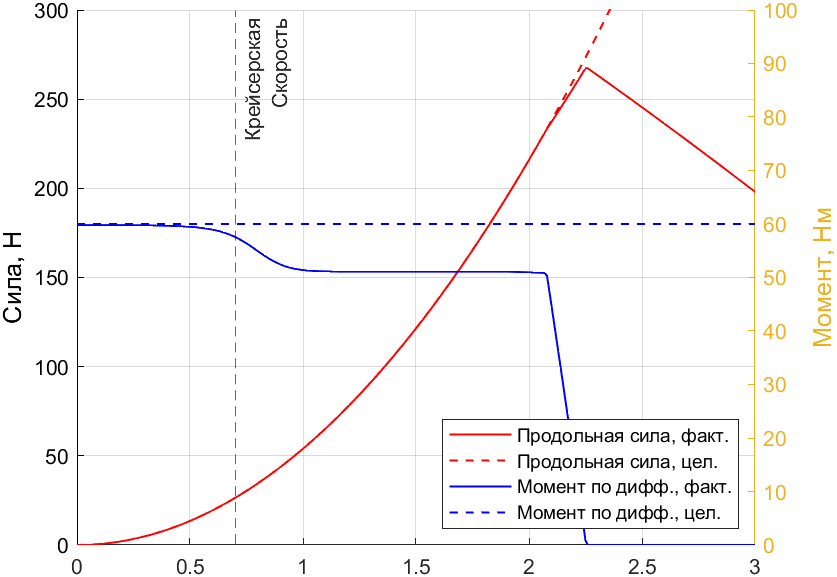
\includegraphics[width=0.8\linewidth]{allocation/Результат - Адаптивный силы.png}
    \caption{Силы и моменты при предлагаемом методе.}
    \label{fig:mmt-300-allocation-optimal-force}
\end{figure}

\section{Структура программного обеспечения для реализации предложенного метода} \label{sec:Allocation/Software}
\begin{noteplan}
	Добавлю структурное описание ПО для реализации метода распределения.
\end{noteplan}

\section{Выводы по главе 4}
\begin{noteplan}
	Выводы что метод позоляет отказоустойчиво распределять управляющее воздействие с учетом подруливающих особенностей ДРК.
\end{noteplan}

\begin{notequestion}
	Надо как-то выйти на то, что используется скорость полученная в третьей главе. Или это уже в финальной главе обьединить?
\end{notequestion}